\chapter{Application of methods}
In following part of thesis is described how to apply discussed methods to our problem. It is necessary to make several adjustments and also combine some of these methods to ensure reliable detections.

\section{Detection pipeline}
Detection is divided into three parts. All three parts are discussed in next three subsections. detection pipeline is visualized in the figure \ref{fig:flowchart}. 

\hspace{5px}
\begin{figure}[H]
\centering
\includegraphics[scale=0.06]{fig/flowchart.pdf}
\caption[Program pipeline]{Visualization of subsequent steps of detection.}
\label{fig:flowchart}
\end{figure}

It can be seen that the symbolic map has two types of inputs. The main advantage of this approach is that it extends the lidar detection range. As we discussed in previous section, used lidar has low vertical resolution - only 16 layers. Thus the bricks are often visible in only one layer of lidar scan. If we use only one scan, there is a high probability of false positive measurements. On the one hand we can decrease the occurrence of false positives by adding other lidar layers into the detection process. But on the other hand two layers are available only from distance smaller than 6 meters and that decreases the detection range. Therefore we exploited both approaches. One layer line segmentation for generating the candidates with low confidence and multilayer pile detector providing high quality estimates.

\section{Line segmentation}
For line segmentation is used IEPF algorithm very similar to the one described in algorithm \ref{alg:segmentation}. Only the final merging parallel segments is omitted, because it can connect two bricks into one. After retrieving the segments, a filtering based on the segment size is done. It is possible to assign the color to the segment because each brick type has unique dimensions. Example of lidar measurement with extracted and filtered lines is in the figure \ref{fig:segments}. Algorithm performance is influenced by correct setup of constants $C$ and $S$ (clustering and splitting distance). If we choose to high C, it could happen that the algorithm joins two bricks into one segment. As described in figure \ref{fig:piledef} the distance between two bricks of same color is 10 cm. Therefore the clustering distance must be always less than 10 cm. If the clustering distance is too low, one brick can be unintentionally divided into many segments and without merging at the end are these segments useless. It is necessary to bear in mind that the lidar precision as shown in table \ref{tab:lidar} is $\pm3$ cm so any clustering with distance smaller than 6 cm will be highly affected be sensor noise. The found segments are transformed into the map frame and passed to symbolic map as low confidence detections. Further are segments passed to pile detector which can filter out false positive detections.

\hspace{8mm}

\begin{figure}[H]
\centering
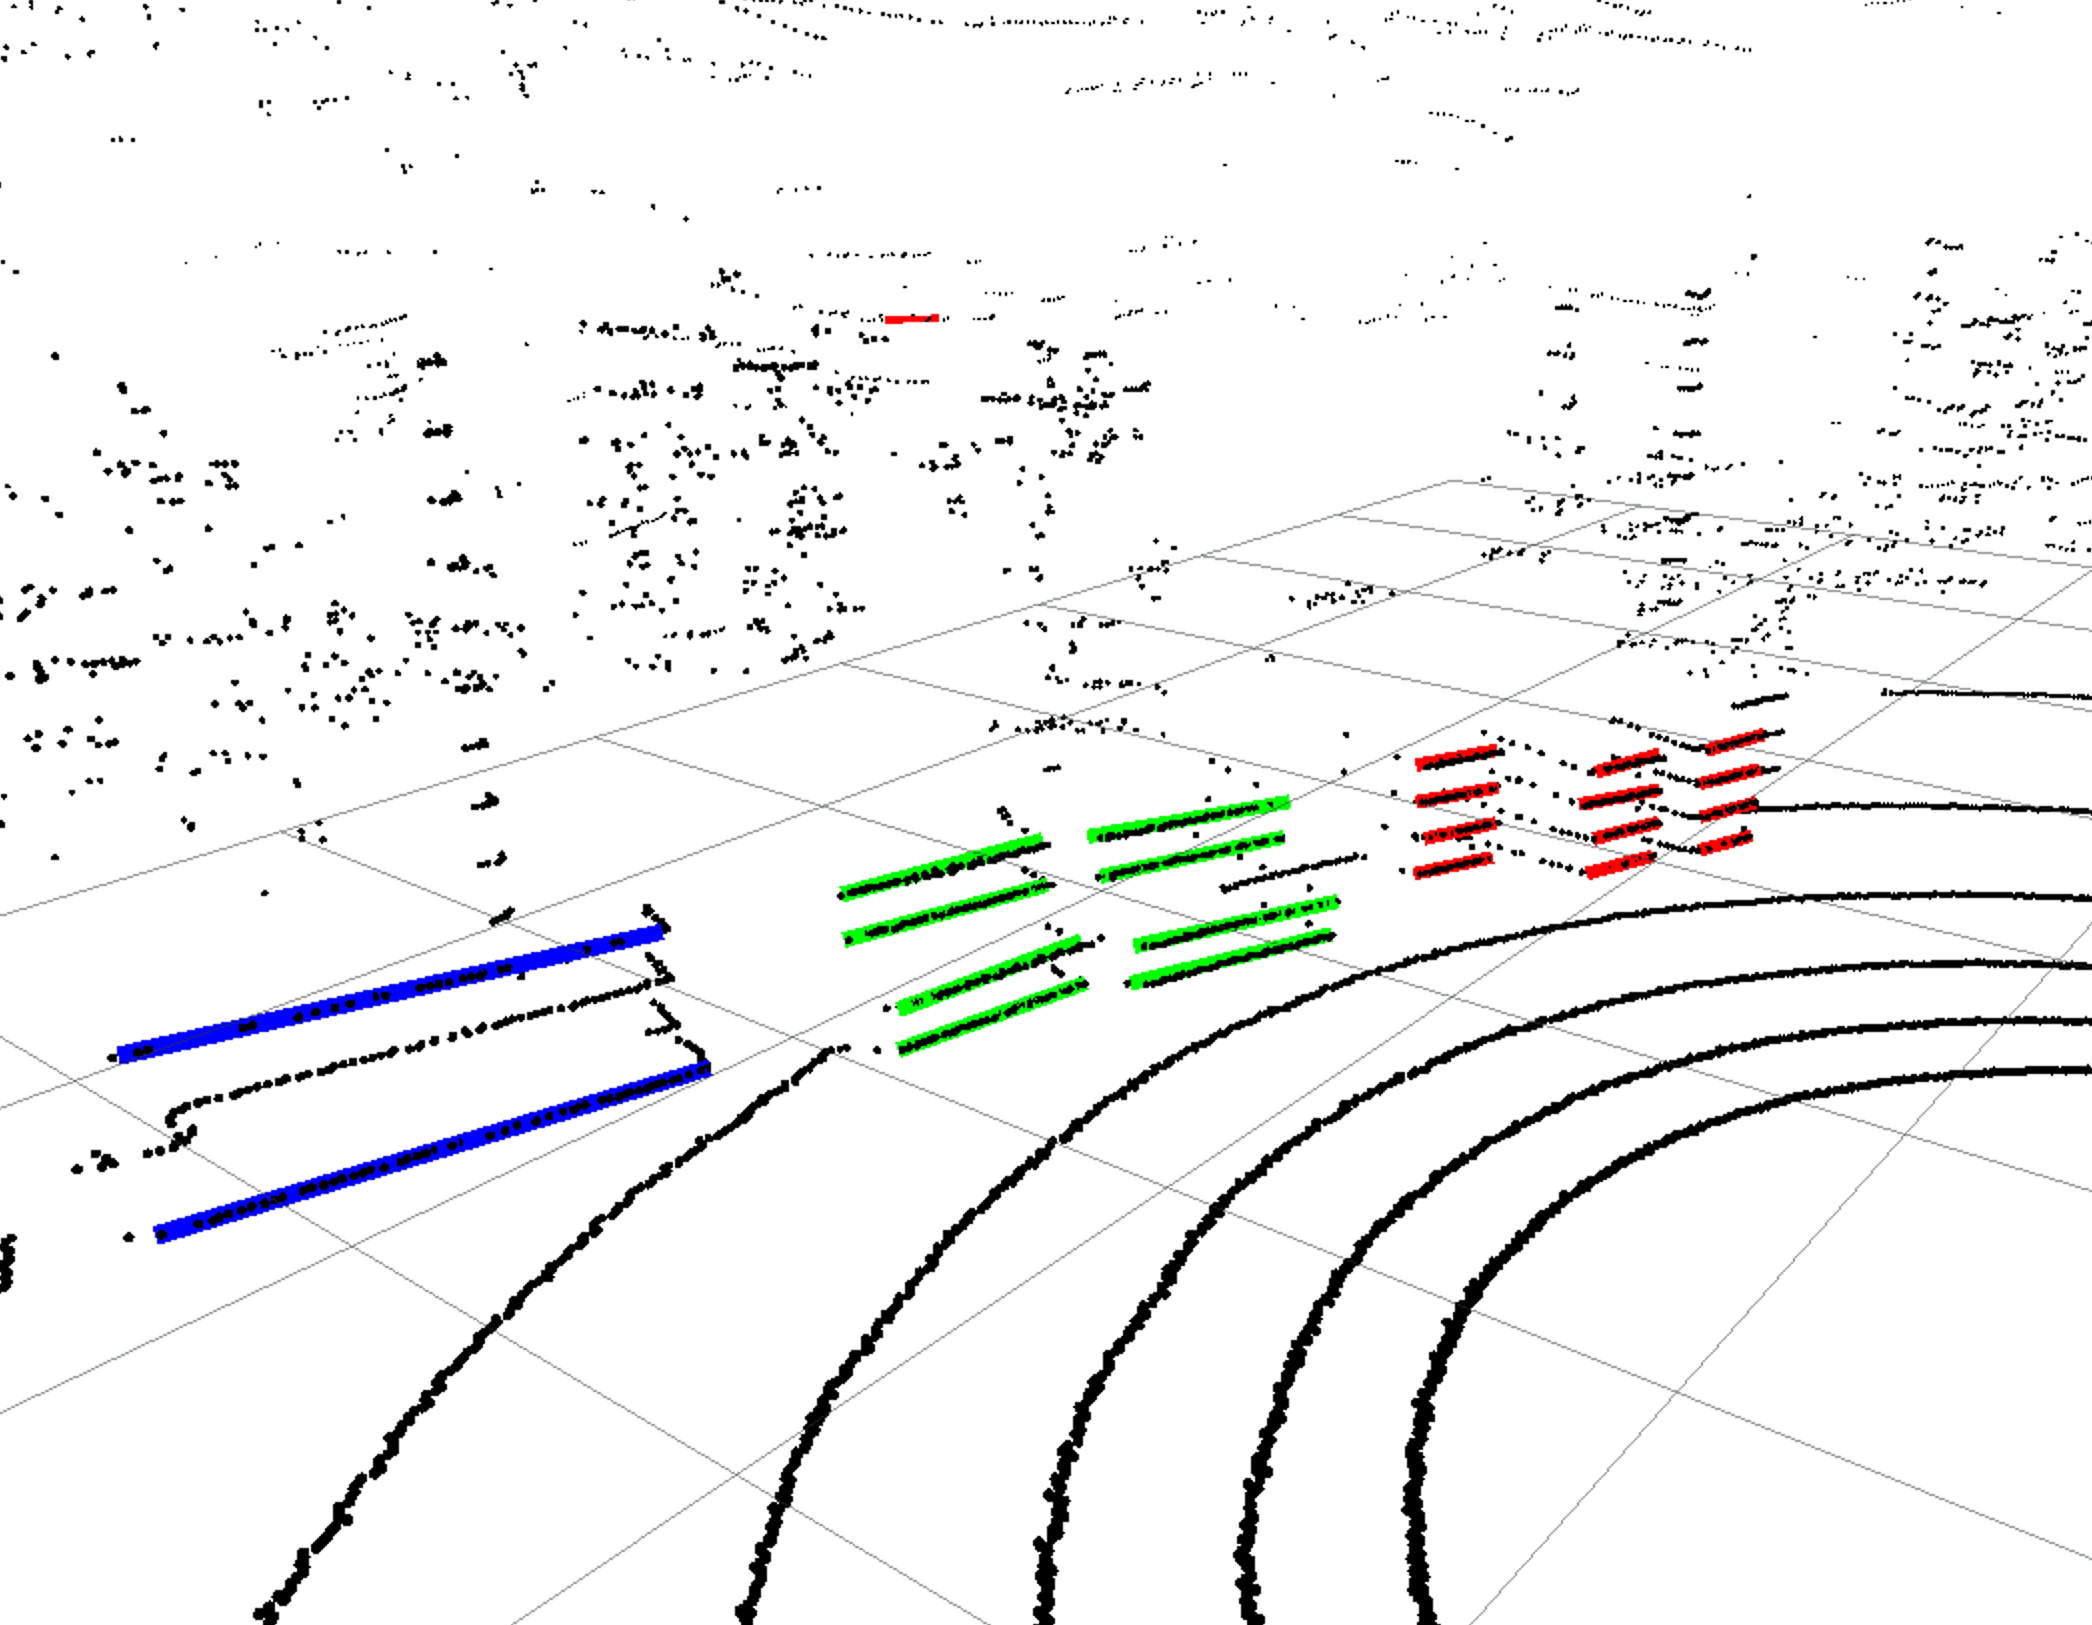
\includegraphics[scale=0.43]{fig/segments}
\caption[Line segmentation visualization]{RViz visualization of line segmentation. In the figure is evident that the bricks are well detected. This detection is done from $\approx3$m. There is visible one false positive detection behind the brick piles on a tree.}
\label{fig:segments}
\end{figure}


\section{Pile detection}
The pile detector uses one of the simplest version of EM algorithm. As a model for the pile is applied 2D multivariete Gaussian distribution with variance fixed to one. Although, this model is not precise description of the detection probability, it has other advantages already discussed in previous chapters. It is easy to work with and it converges to the global optimum very well. Only the mean value is optimized and it should converge into the center of the pile. The stopping criterion for the algorithm is solely number of iterations. The robot is realtime system and there are strict demands for meeting a deadline. There are further requirements for a hypothesis to be declared as pile after the optimization is done. We look around the proposed center in one meter radius and we inspect all bricks found in this area. All the following conditions must be fulfilled for segments in the pile:
\begin{itemize}
\item There are at least two unique heights ($z$ positions).
\item There are at least two unique places ($(x,y)$ positions).
\item Difference between maximal and minimal height is less than the pile height.
\item Pile center is inside the arena.
\end{itemize}
When these conditions are met then the hypothesis is declared as pile and pushed into symbolic map with high confidence. When one of these conditions is violated then all the segments in this hypothesis are deleted and the algorithm runs again until there are no more segments within the hypothesis radius. Second condition does not apply to the orange pile. Whole procedure is shown in algorithm \ref{alg:pile_detection}.

\begin{algorithm}[]
 \KwData{segments}
 \KwResult{pile\_position}
\While{True}{
	pile\_position = fit\_em(segments)\;
	pile\_segments = segments\_in\_pile(pile\_position, segments)\;
	\If{pile\_segments.size() $< 2$}{
		return None\;	
	}
	\eIf{is\_pile(pile\_segments)}{
		return pile\_position\;
	}{
		segments.delete(pile\_segments)\;
	}
} 
 \caption{Algorithm to obtain pile centers.}
 \label{alg:pile_detection}
\end{algorithm}

\begin{figure}[H]
\centering
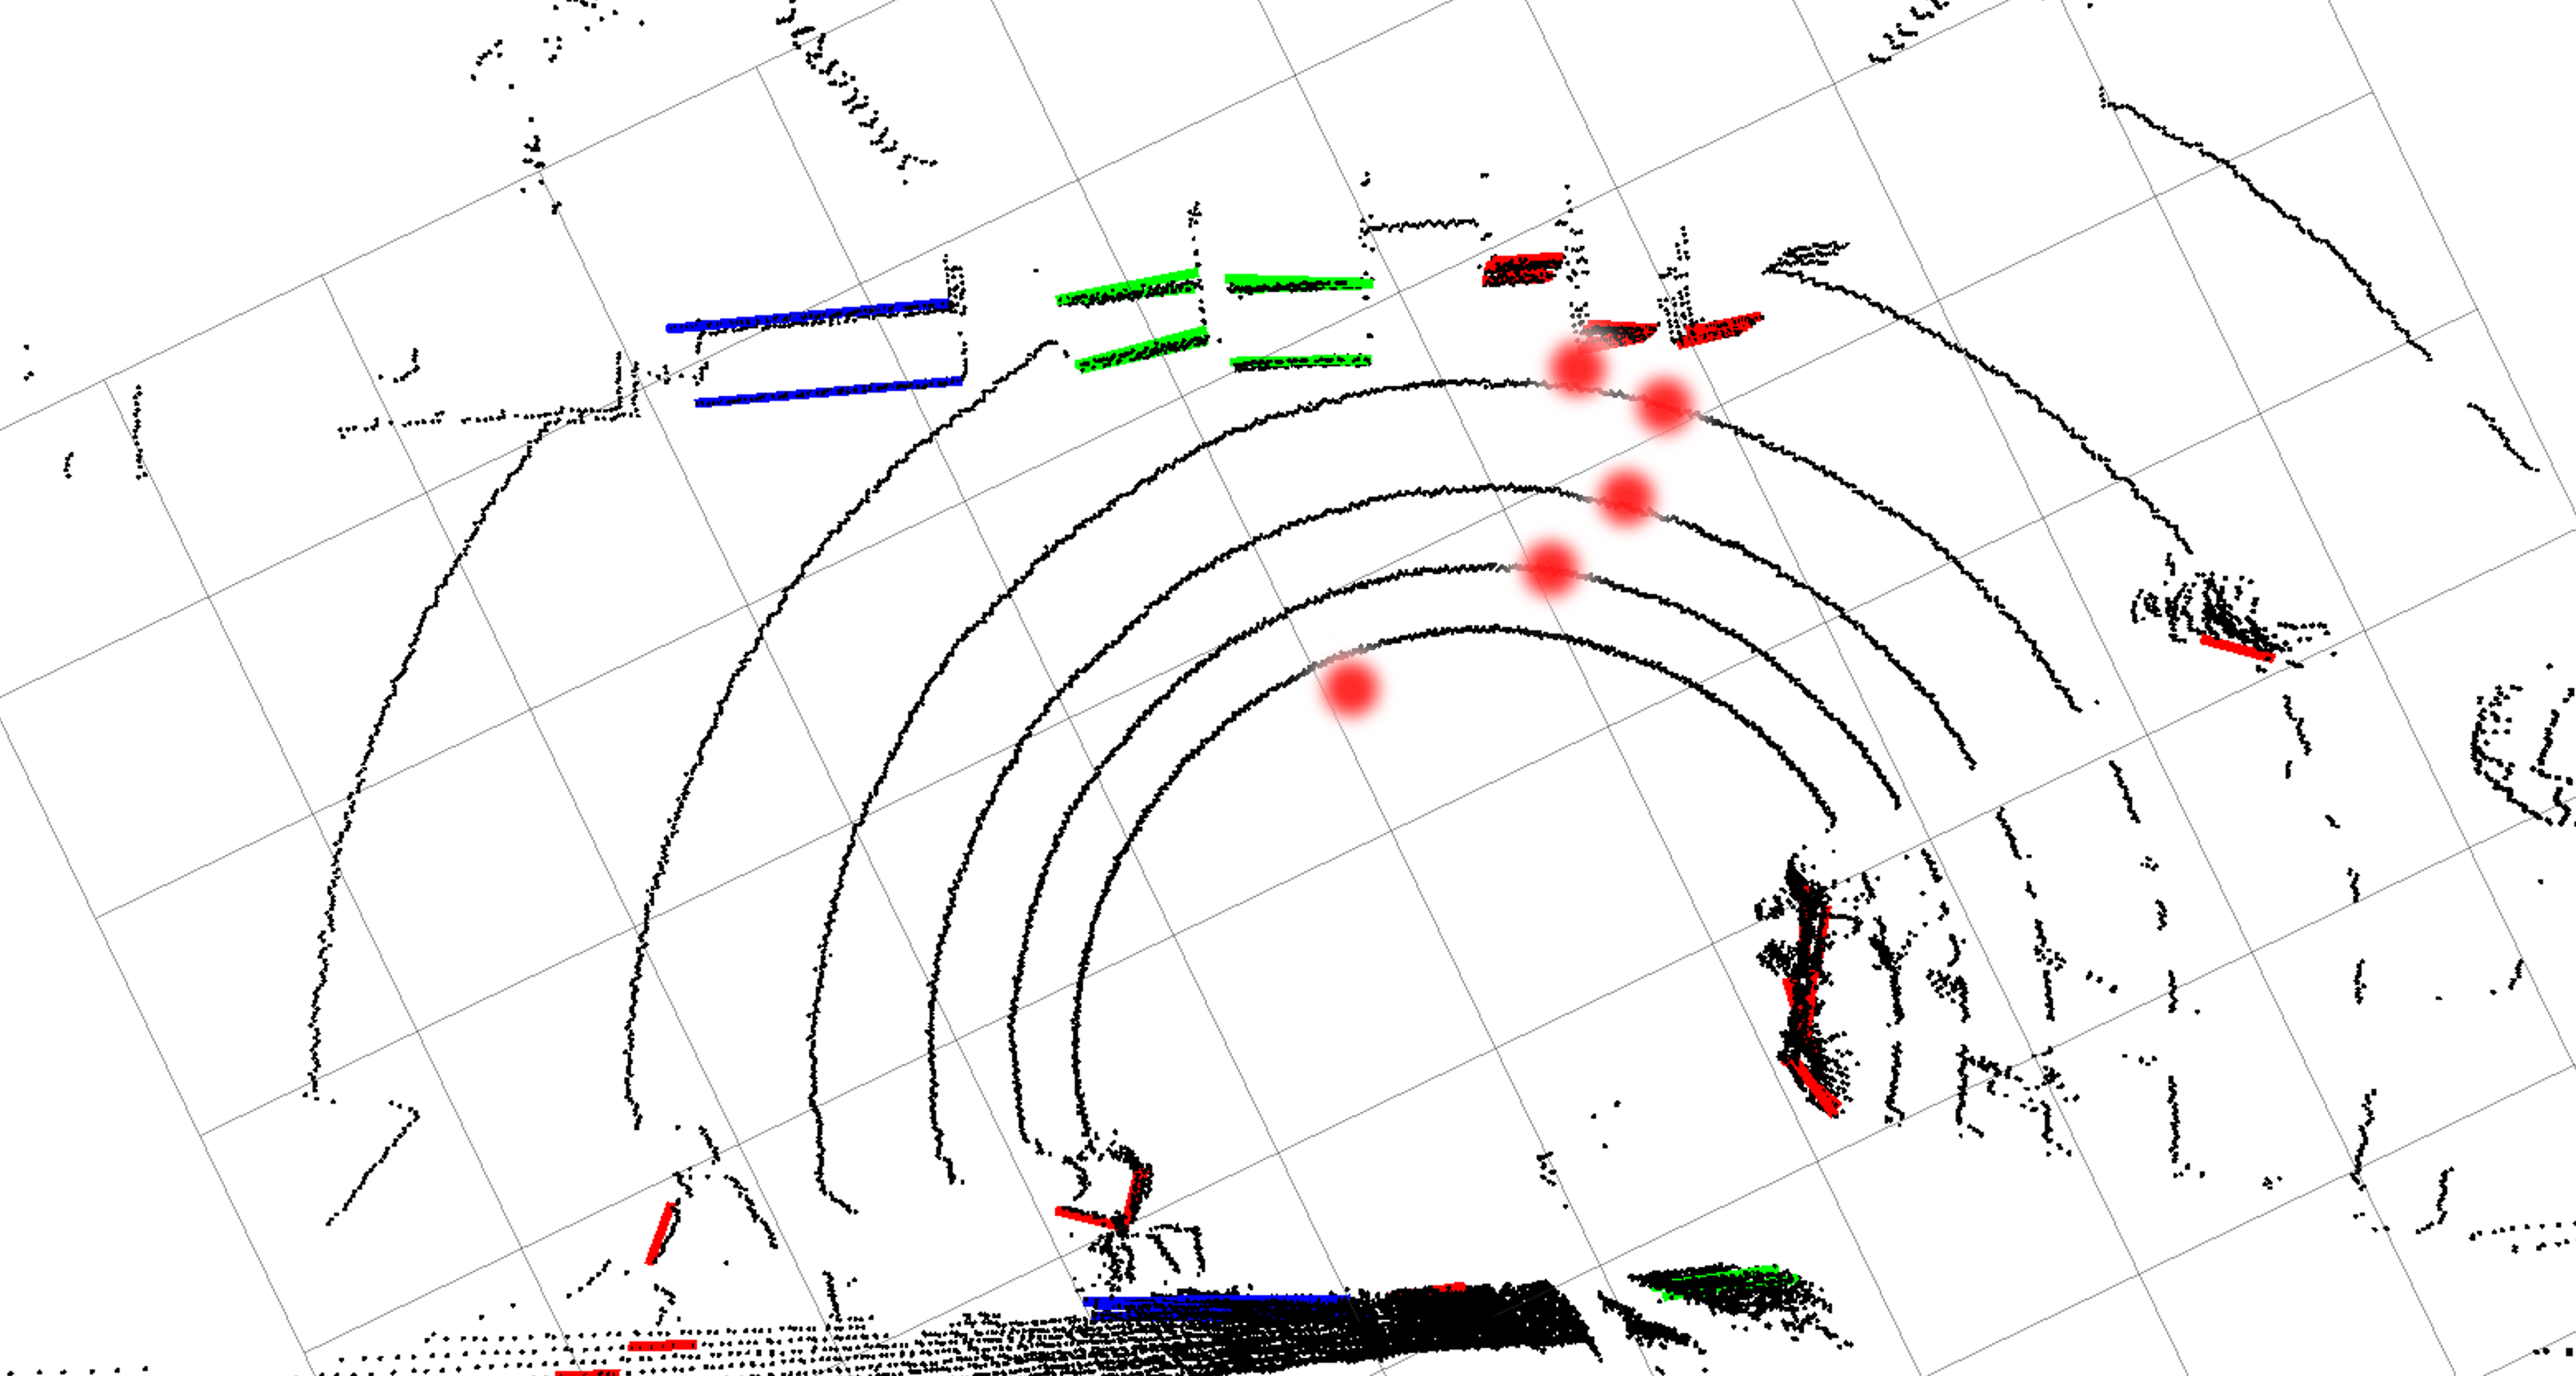
\includegraphics[scale=0.3]{fig/em_algo.png}
\caption[Em Algorithm in pile detector]{Several steps of EM algorithm for the red pile. Colored lines are the visualized segments same as in the figure \ref{fig:segments}. Red dots show subsequent positions of mean value of multivariete Gaussian. Although, there are many false positives especially in the bottom of the picture, the pile model ensures that the algorithm converges to correct place.}
\label{fig:em}
\end{figure}


\section{Pattern fitting}
Ah shown in the figure \ref{fig:flowchart} the last step of detection pipeline is pattern fitting. It is also visible that there are two types of input into this last step. Each input is used for different type of pattern fitting. In previous two sections it was described how to generate candidates with different levels of confidence. This section describes how the candidates can be used for generating actual positions and how information about the spatial distribution of bricks can be exploited for the detection. From figure \ref{fig:piledef} is known exact position of each pile and even each brick. Pattern in which are bricks stacked has three degrees of freedom - position $(x, y)$ and rotation $\phi$. Goal of the pattern fitting is to find values of these parameters in the map frame.

\subsection{Brick fitting}
The first type of fitting is using detected 3D positions of individual bricks obtained in pile detector. In the pattern is described position of each brick which can be detected by lidar sensor. Next step is to generate hypothesis which align this pattern with the measured positions of bricks. For this step is utilized the RANSAC algorithm. Firstly we draw two different bricks from detected set of bricks. Secondly the correspondences are used to find the transformation - two correspondences are enough to generate the hypothesis (rotation matrix $R$ and translation vector $t$). The brick types (colors) and brick $z$ positions are used as the correspondences. Also we know that the distance between corresponding pairs should match, otherwise it would be incorrect correspondence. Lastly we measure the cost of the hypothesis. When the bricks are stacked into the pattern with a reasonable precision, it is possible to fit the pile with average brick error down to $\pm 3$cm. After such a observation we set the inlier distance to $5$cm. Algorithm is stopped after certain number of iterations. The result is passed only if all detected bricks are inliers.

\subsubsection{Hypothesis ambiguity}
It is obvious that we cannot properly test the hypothesis when there are not enough bricks found. In addition we can see the pile from behind which renders a two different patterns to match. For this reason is required at least five detected red bricks to even start the brick fitting. As shown in the figure \ref{fig:ambiguity} even with four detected red bricks can be hypothesis easily fitted incorrectly. All conditions which can start fitting the hypothesis from front view are listed bellow:
\begin{itemize}
\item 5 red bricks detected.
\item 3 green bricks detected.
\item 4 bricks of at least two colors detected.
\end{itemize}
For view from behind is sufficient only the last condition.
\begin{figure}[H]
\centering
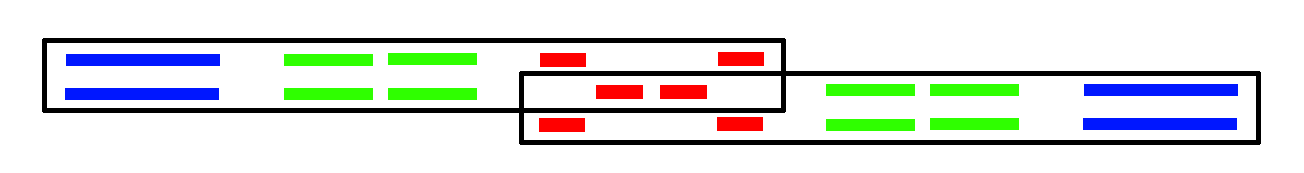
\includegraphics[scale=0.3]{fig/ambiguous.png}
\caption[Hypothesis ambiguity]{In black rectangles are visualized two possible hypothesis which can be generated by four red bricks in the intersection of rectangles. This is top view of detection from the front, so it is not visible that all red bricks are in two layers.}
\label{fig:ambiguity}
\end{figure}

\subsection{Cluster fitting}
The second type of fitting polls clusters from symbolic map and utilizes their confidence and spatial distribution. For RANSAC algorithm would be hypothesis using only four clusters too sparse to fit reliably. Because of this reason is the cluster fitting done by the EM algorithm. As in pile detection is used multivariete Gaussian distribution to represent the pile but this time the model takes in account relationships between positions of the piles. We define the probability model as follows:
\begin{equation}
P(\vec{x}_m) = \mathcal{N}_m(\vec{x}_m; \vec{\mu} + k_m\vec{v}; \bm{\Sigma}),
\label{eq:prob}
\end{equation}
where $m$ is pile (color) index and $M$ is absolute number of colors, $\vec{x}_m$ is measurement of color $m$, $\vec{\mu}$ is mean value of whole model, $\bm{\Sigma_m}$ is covariance matrix, $k_m$ is scalar multiplier unique for each pile and $\vec{v}$ is defined as:
\begin{equation}
\vec{v} = \begin{bmatrix}
\cos \phi \\
\sin \phi
\end{bmatrix},
\end{equation}
where $\phi$ is rotation of model. This definition of model ensures that all piles (Gaussians) are in the line with distance defined by multiplier $k$. Now we want to obtain the position and rotation of such a model based on real measurements. There is a closed form solution for maximizing both terms which can be found using maximum likelihood estimate. For mean value is derivation very similar to multivariete Gaussian:
\begin{align}
\frac{\partial \log\mathcal{L} }{\partial \vec{\mu}_m} &=  \bm{\Sigma}^{-1}_m \sum_{n = 1}^{N_m} (\vec{x}_{m_n} - \vec{\mu} - k_m \vec{v}) \\
\vec{\mu_m} &= \sum_{n = 1}^{N_m} \frac{\vec{x}_{m_n} - k_m \vec{v}}{N_m}.
\end{align}
Further is necessary to derive MLE for rotation $\phi$ which is hidden inside vector $\vec{v}$. For simplicity is now the matrix equation split into one part for each of two dimensions.  
\begin{align}
\frac{\partial \log\mathcal{L}_x }{\partial \phi_m} &= \frac{1}{\sigma^2_x} \sum_{n=1}^{N_m} (x_{m_n, x} - \mu_x - k_{m, x} \cos \phi) \left( -k_{m,x} \sin \phi\right)  \\
\frac{\partial \log\mathcal{L}_y }{\partial \phi_m} &= \frac{1}{\sigma^2_y} \sum_{n=1}^{N_m} (x_{m_n, y} - \mu_y - k_{m, y} \sin \phi) k_{m,y} \cos \phi
\end{align}
Likelihood derivative is now set equal to zero to find the extremes for each dimension.
\begin{align}
\cos \phi_m &= \frac{1}{k_{m, x}N_m} \sum_{n = 1}^{N_m} x_{m_n, x} - \mu_x \\ 
\sin \phi_m &=  \frac{1}{k_{m, y}N_m} \sum_{n = 1}^{N_m} x_{m_n, y} - \mu_y .
\end{align}
Now it is possible divide one equation by the other, use basic relationship of trigonometric functions and derive final expression for maximizing the rotation $\phi$:
\begin{align}
\phi_m &= \arctan \left( \frac{\dfrac{\sum_{n = 1}^{N_m} \left( x_{m_n, y} - \mu_y \right)}{k_{m, y}N_m} }{ \dfrac{\sum_{n = 1}^{N_m} \left( x_{m_n, x} - \mu_x \right)}{k_{m, x}N_m} }\right).
\end{align}
Although the expression can be further simplified, in this form it is easier to weight each data sample by the expectation $\alpha$. In addition is necessary to consider contribution of each color to pile model. This can be done in two ways. One possibility is to set equal contribution to each data sample. In our case this could lead to bias towards the most detected color (usually red). Thus we set equal contribution to each color instead of data sample. Final form used in maximization step looks as follows:
\begin{align}
\vec{\mu} =& \sum_{m=1}^M \dfrac{\sum_{n = 1}^{N_m}  \vec{\gamma}_{m_n} \left( \vec{x}_{m_n} - k_m \vec{v} \right) }{M} \\
\phi = \arctan & \left( \dfrac{\sum_{m=1}^{M} \dfrac{\sum_{n = 1}^{N_m} \gamma_{m_n, y}(x_{m_n, y} - \mu_y)}{k_{m, y} } }{\sum_{m=1}^{M} \dfrac{\sum_{n = 1}^{N_m} \gamma_{m_n, x} (x_{m_n, x} - \mu_x) }{k_{m, x}} }\right).
\end{align}
Method is demonstrated in the figure \ref{fig:em_pattern}. Expectation is calculated simply by evaluating the probability of sample $P(\vec{x}_m)$ as in equation \ref{eq:prob}. Results can be further improved when the confidence of sample is used as the prior probability.

\begin{figure}[H]
	\centering
	\begin{subfigure}{0.49\textwidth}
		\centering
		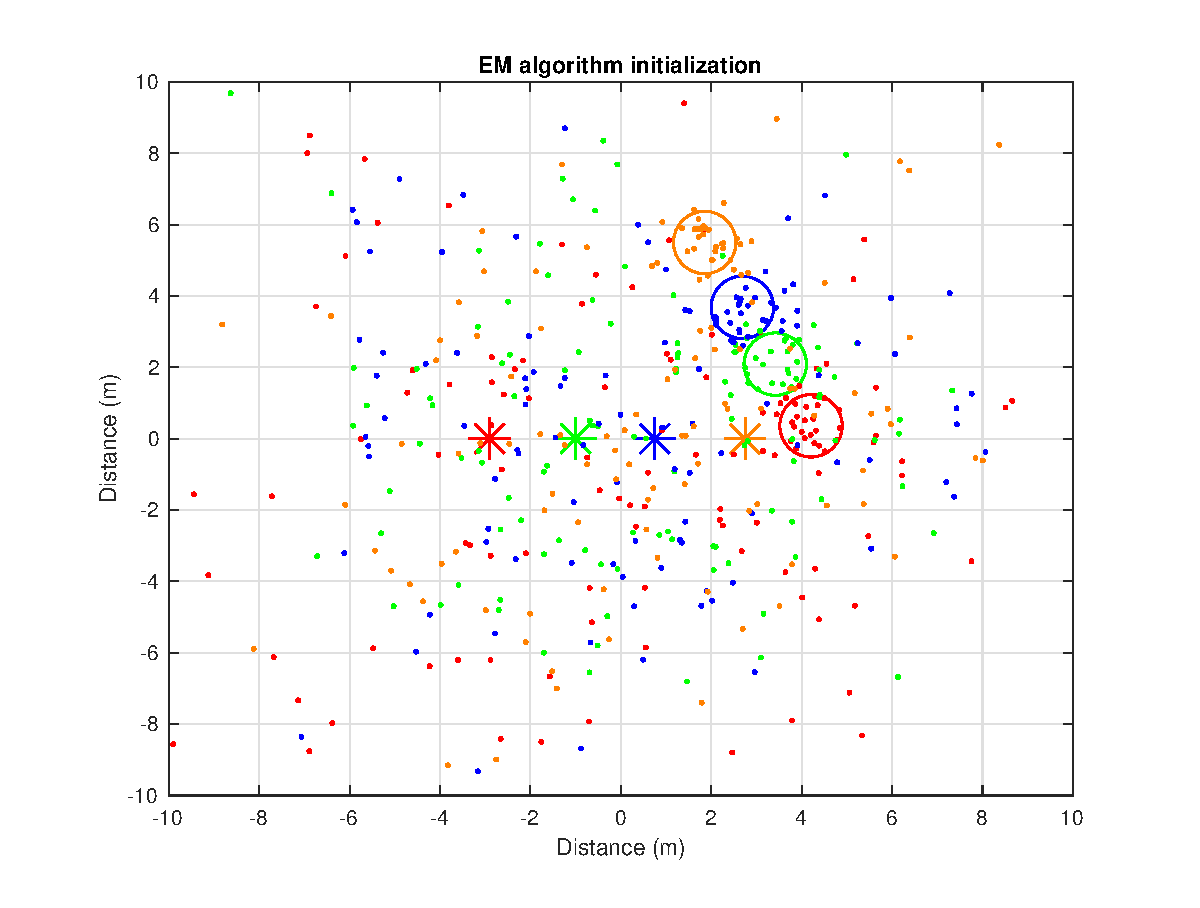
\includegraphics[scale=0.43]{fig/em_init.eps}
	\end{subfigure}
	\begin{subfigure}{.49\textwidth}
		\centering
		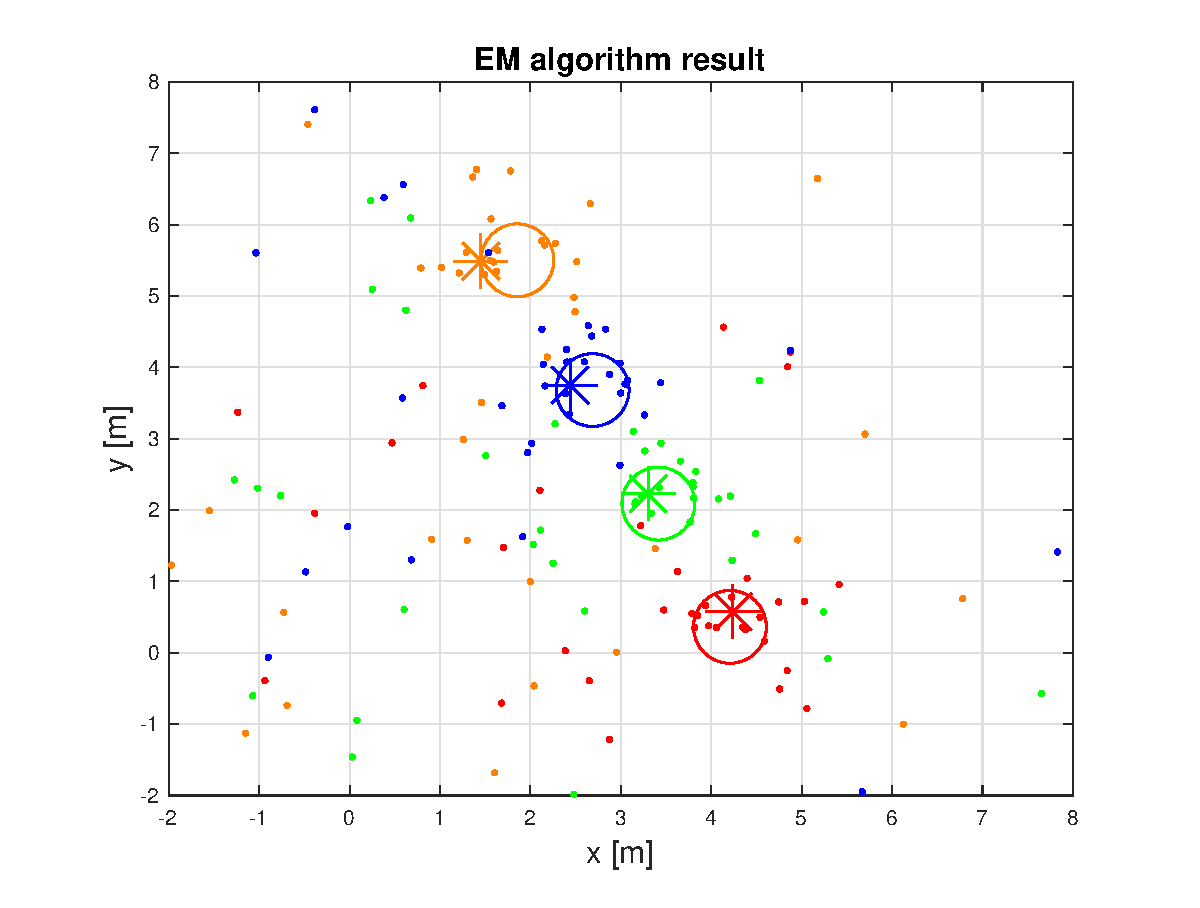
\includegraphics[scale=0.43]{fig/em_result.eps}

	\end{subfigure}
	
	\caption[EM pattern fitting]{In the pictures is visualised pattern fitting using EM algorithm. On the left is algorithm initialized with parameters $\vec{x}=(0, 0)$ and $\phi=0$. Algorithm estimate is marked by stars. Points are generated by sampling multivariete Gaussian distribution. Model was sampled with parameters $\vec{x}=(3, 3)$ and $\phi=2$ to create desired pattern of points. Positions of sampled piles are marked as circles. At the end of process are parameters found correctly.}
	\label{fig:em_pattern}
\end{figure}

\subsubsection{Convergence}
The unimodality of model's likelihood was disrupted by adding the rotation parameter to Gaussians. Possible local optimum is shown in the figure \ref{fig:em_local}. Now there are no guarantees that the algorithm will converge into the global optimum. This is common issue of EM algorithm when dealing with more complex problems. Many solutions of this issue was proposed. Very advantageous is that local optima are usually significantly worse in terms of likelihood than the global optimum. One of methods how to avoid local optima is the deterministic annealing which influences how the expectation is used in maximization step \cite{ueda1998}. Another way how to escape local optimum is to apply the perturbations to parameters of model. In our case it could be for example rotating the model by $180\degree$. Different approach would be population based em algorithm with multiple initializations or informed initialization. The latter is easily applicable in our case because the confidences of clusters could be used in the expectation step. Because we have the formulas for gradient it is also possible to use arbitrary gradient ascend method instead of EM algorithm to maximize likelihood of the model.

\begin{figure}[H]
	\centering
	\begin{subfigure}{0.49\textwidth}
		\centering
		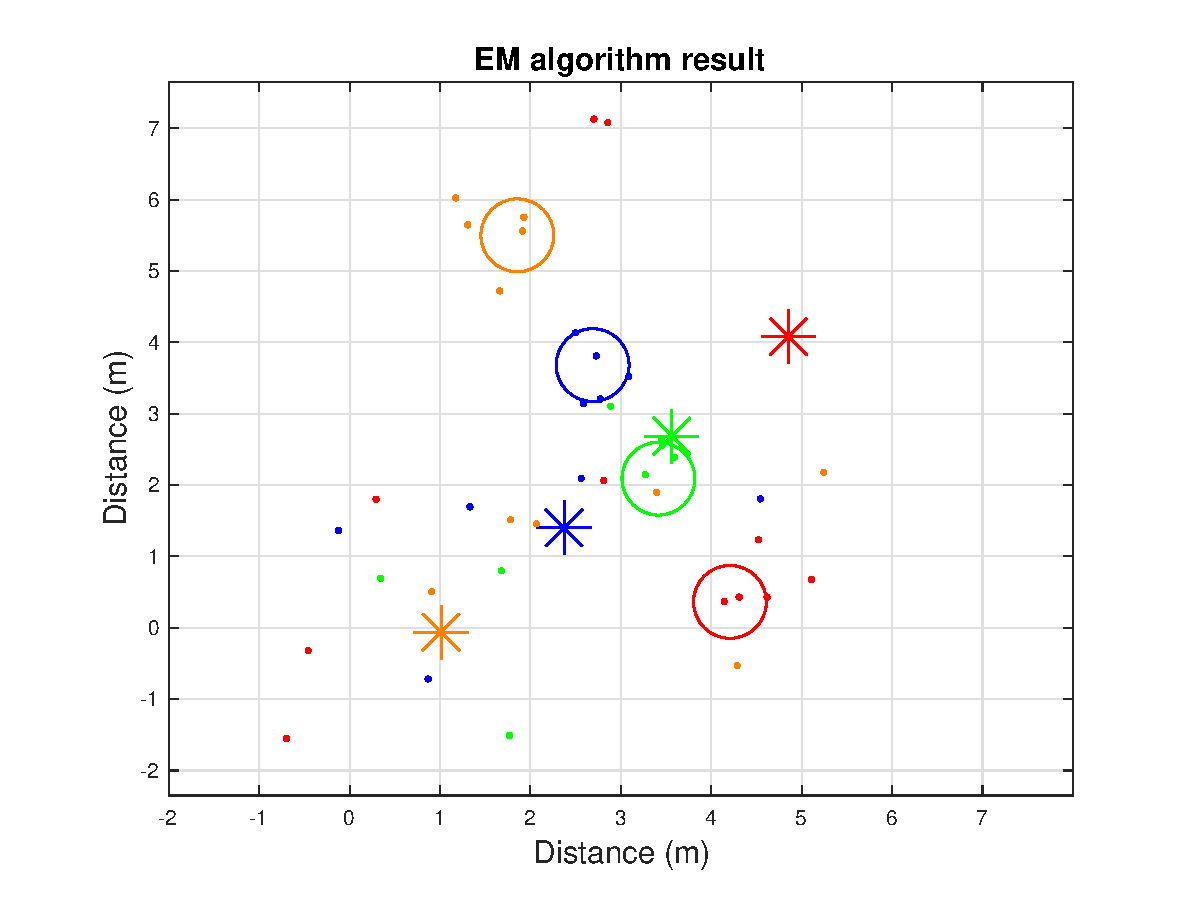
\includegraphics[scale=0.43]{fig/em_local.eps}
	\end{subfigure}
	\begin{subfigure}{.49\textwidth}
		\centering
		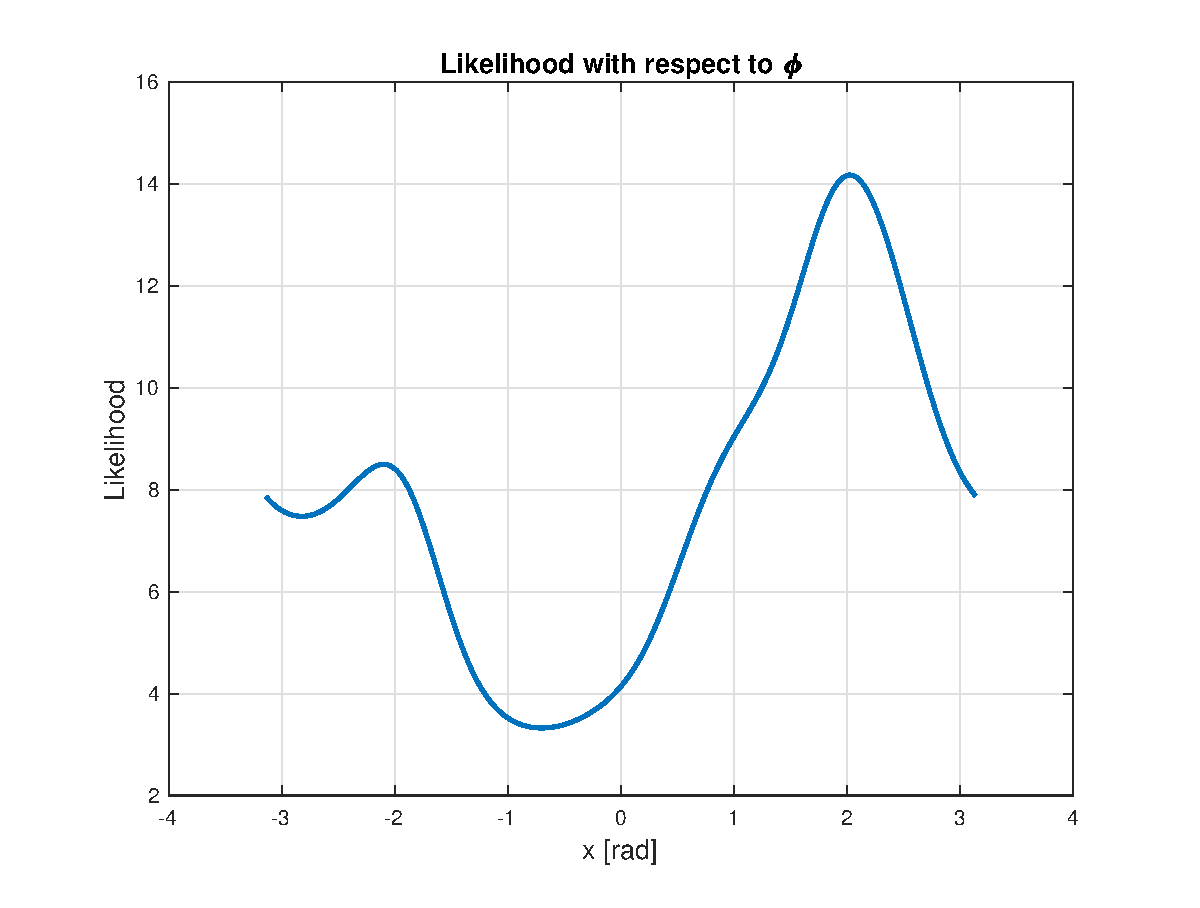
\includegraphics[scale=0.43]{fig/em_local_chart.eps}
		
	\end{subfigure}
	
	\caption[EM local optima]{When there is not enough samples the EM algorithm is more susceptible to ending in local optima as shown on the left. Right picture shows how different rotations of model with fixed mean influences the likelihood and it also shows that there is a local maximum. The likelihood is maximal when $\phi = 2$ which is optimal rotation of model.}
	\label{fig:em_local}
\end{figure}

\section{Arena exploration}
It is vital to emphasize on proper arena exploration. If all the interest points are not found, the robot can not proceed in completing of the challenge. Except the initial brick position is necessary to find also the destination where the bricks should be placed. This place is marked by checker pattern in the figure \ref{fig:checker}. Only sensor which can detect the destination pattern is camera. The big advantage is that the camera is mounted onto the arm so that it can be raised into height and turn around. As can be seen in the figure \ref{fig:detection_range} the most limiting factor of the detection range is currently the destination pattern search.

\begin{figure}[H]
	\centering
	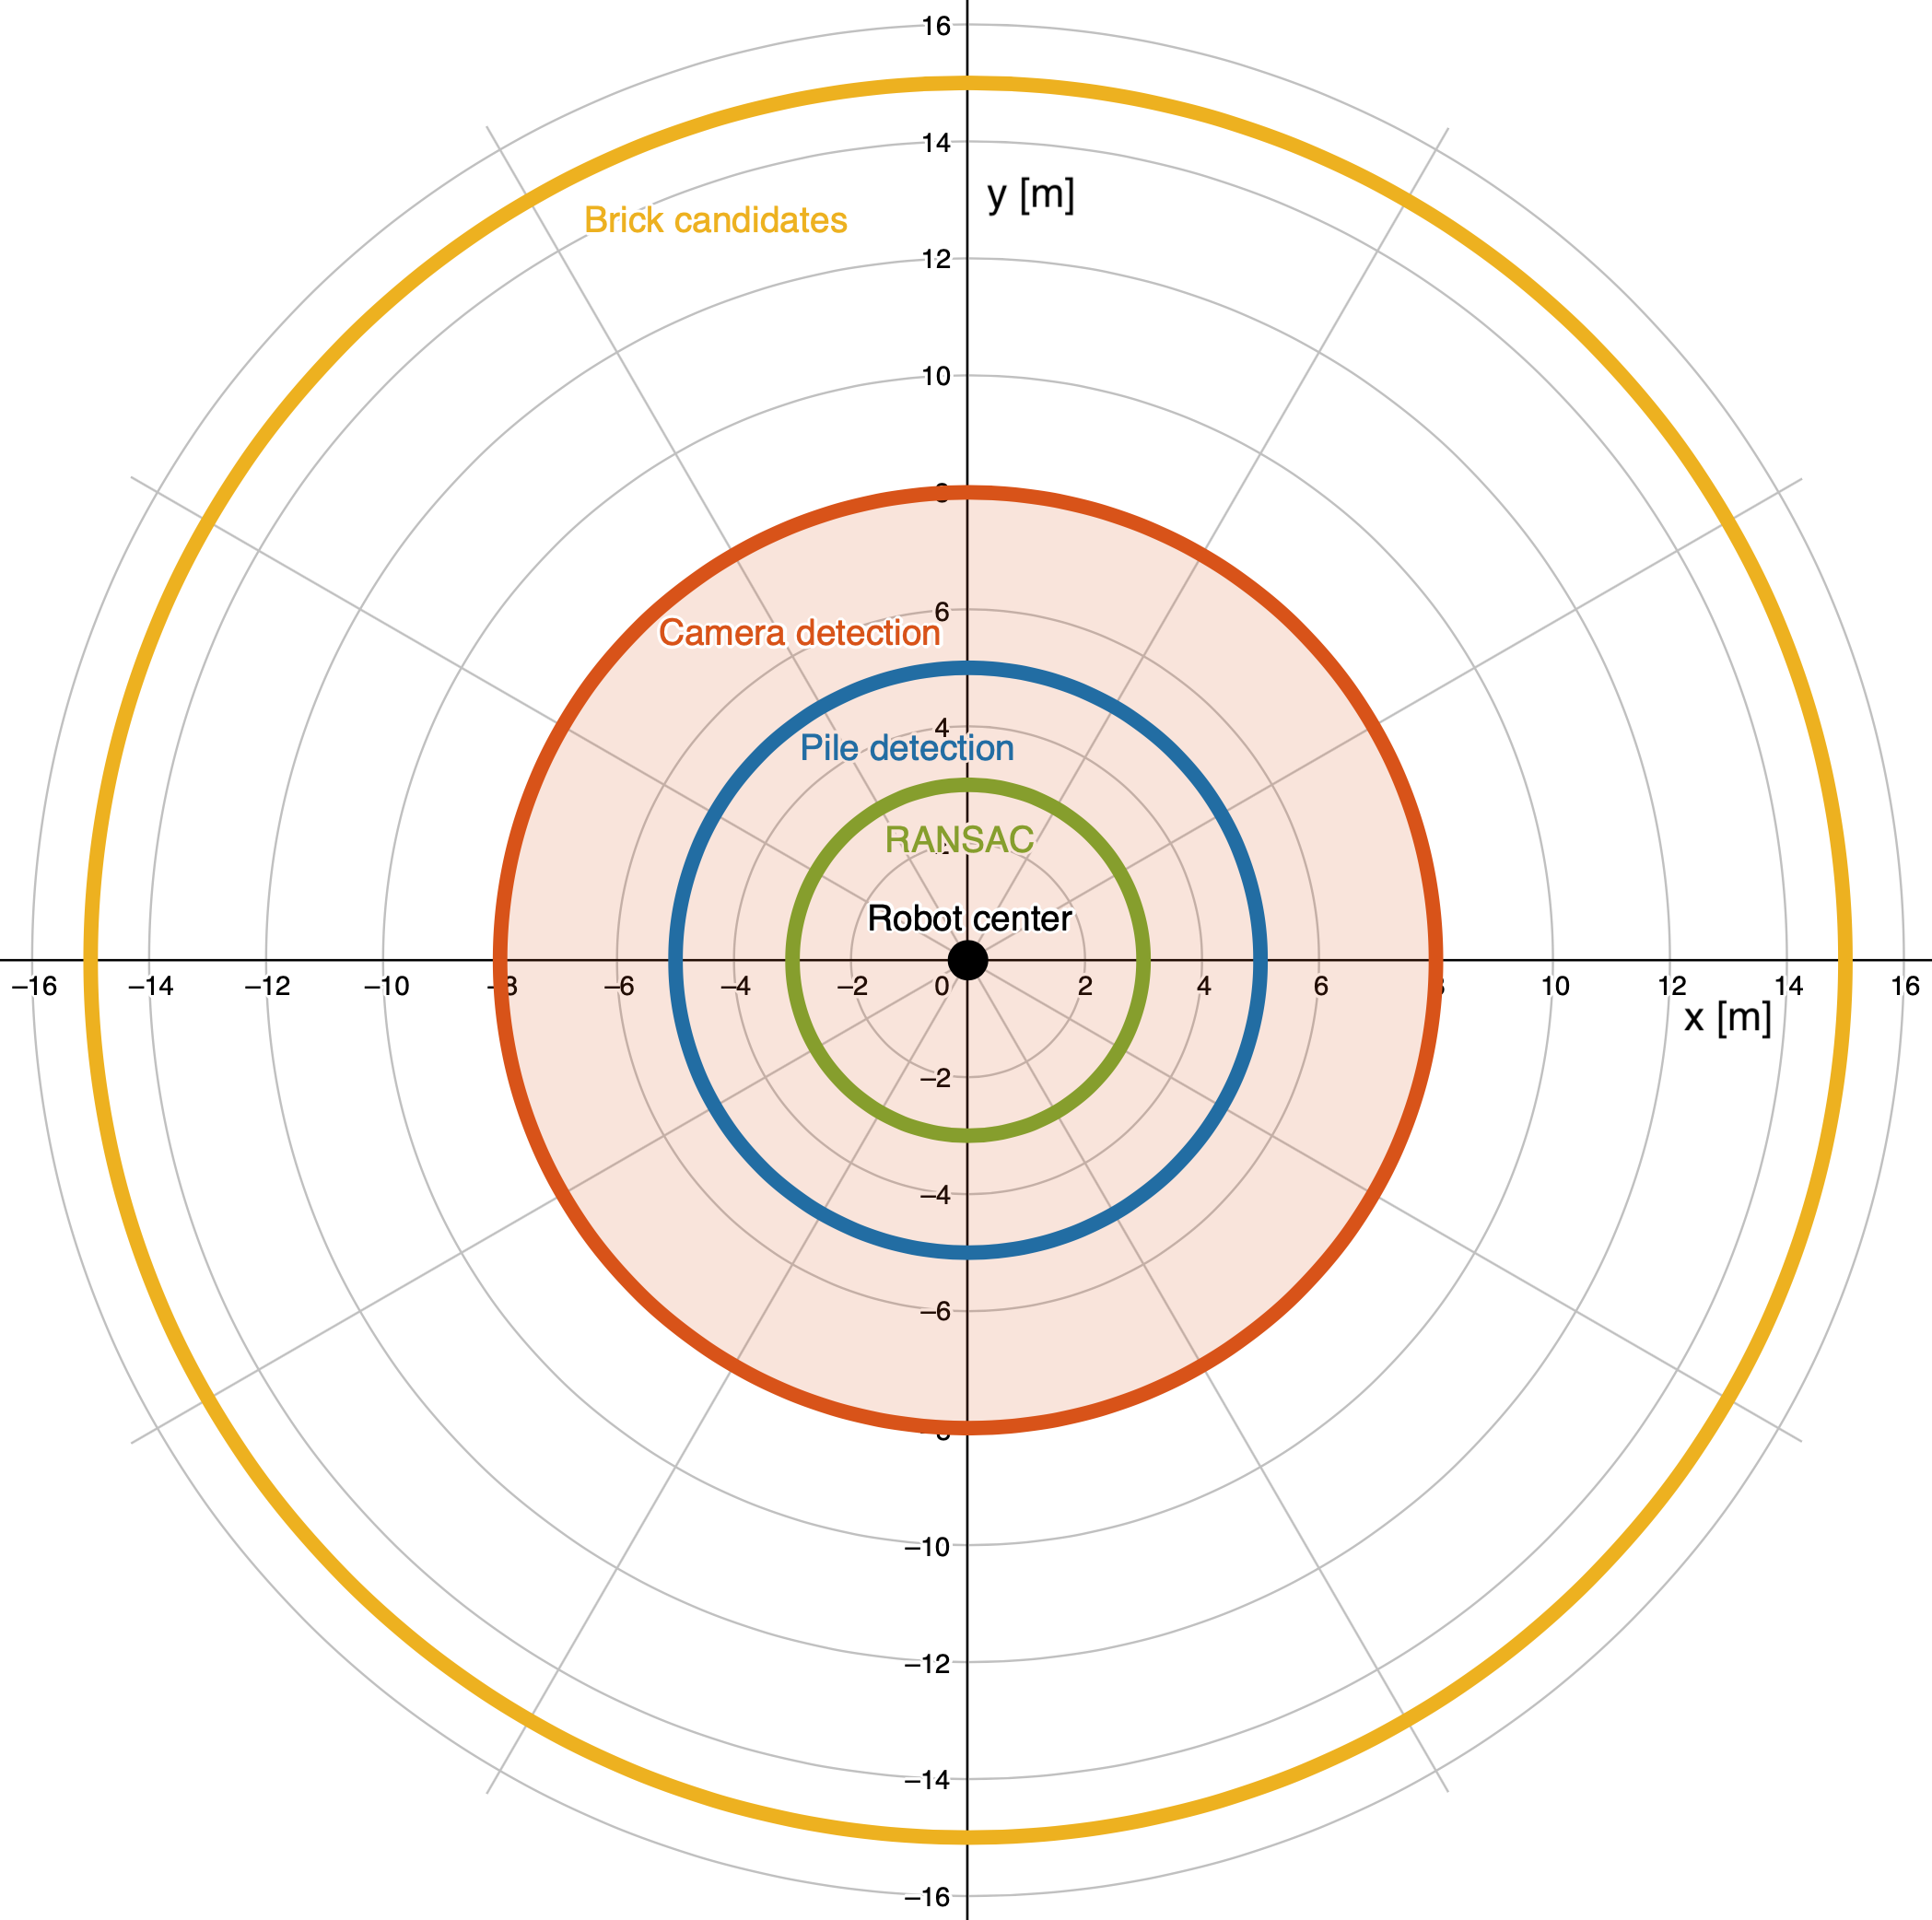
\includegraphics[scale=0.38]{fig/detection_range.png}
	\caption[Detection ranges]{In the picture we see the range of each type of detection. Fit the complete hypothesis using RANSAC method (green) requires high number of segments in piles, so the range is around $3$m. For detection of the pile (blue) is required just few segments - the detection range is roughly $5$m. Camera can obtain candidates for checker pattern (red) from maximal distance of $8$m, that is the limit distance for are exploration. From even bigger distance can be generated candidates for bricks (yellow) using the lidar sensor. The upper boundary can be even higher but we set it manually to $15$m to reduce the number of false positive detections.}
	\label{fig:detection_range}
\end{figure}

 The waypoints of exploration movement should be generated so that the area of whole arena is covered by circles with 8 meter radius. Generated waypoints in the arena are visualized in the figure \ref{fig:map_annot}. On each waypoint the robot must stop, raise the arm and look around with camera. There are several reason while camera detection cannot be done while moving. First of all the arm can not be raised to the highest possible position while the robot is moving, otherwise it could get stuck or damaged. In addition the motion blur of image would reduce the detection range even further. Although, during camera detection the robot must be still, the lidar detections can be done while moving, which further improves the detection. Whole map exploration is described in the algorithm \ref{alg:exploration}.

\begin{figure}[H]
	\centering
	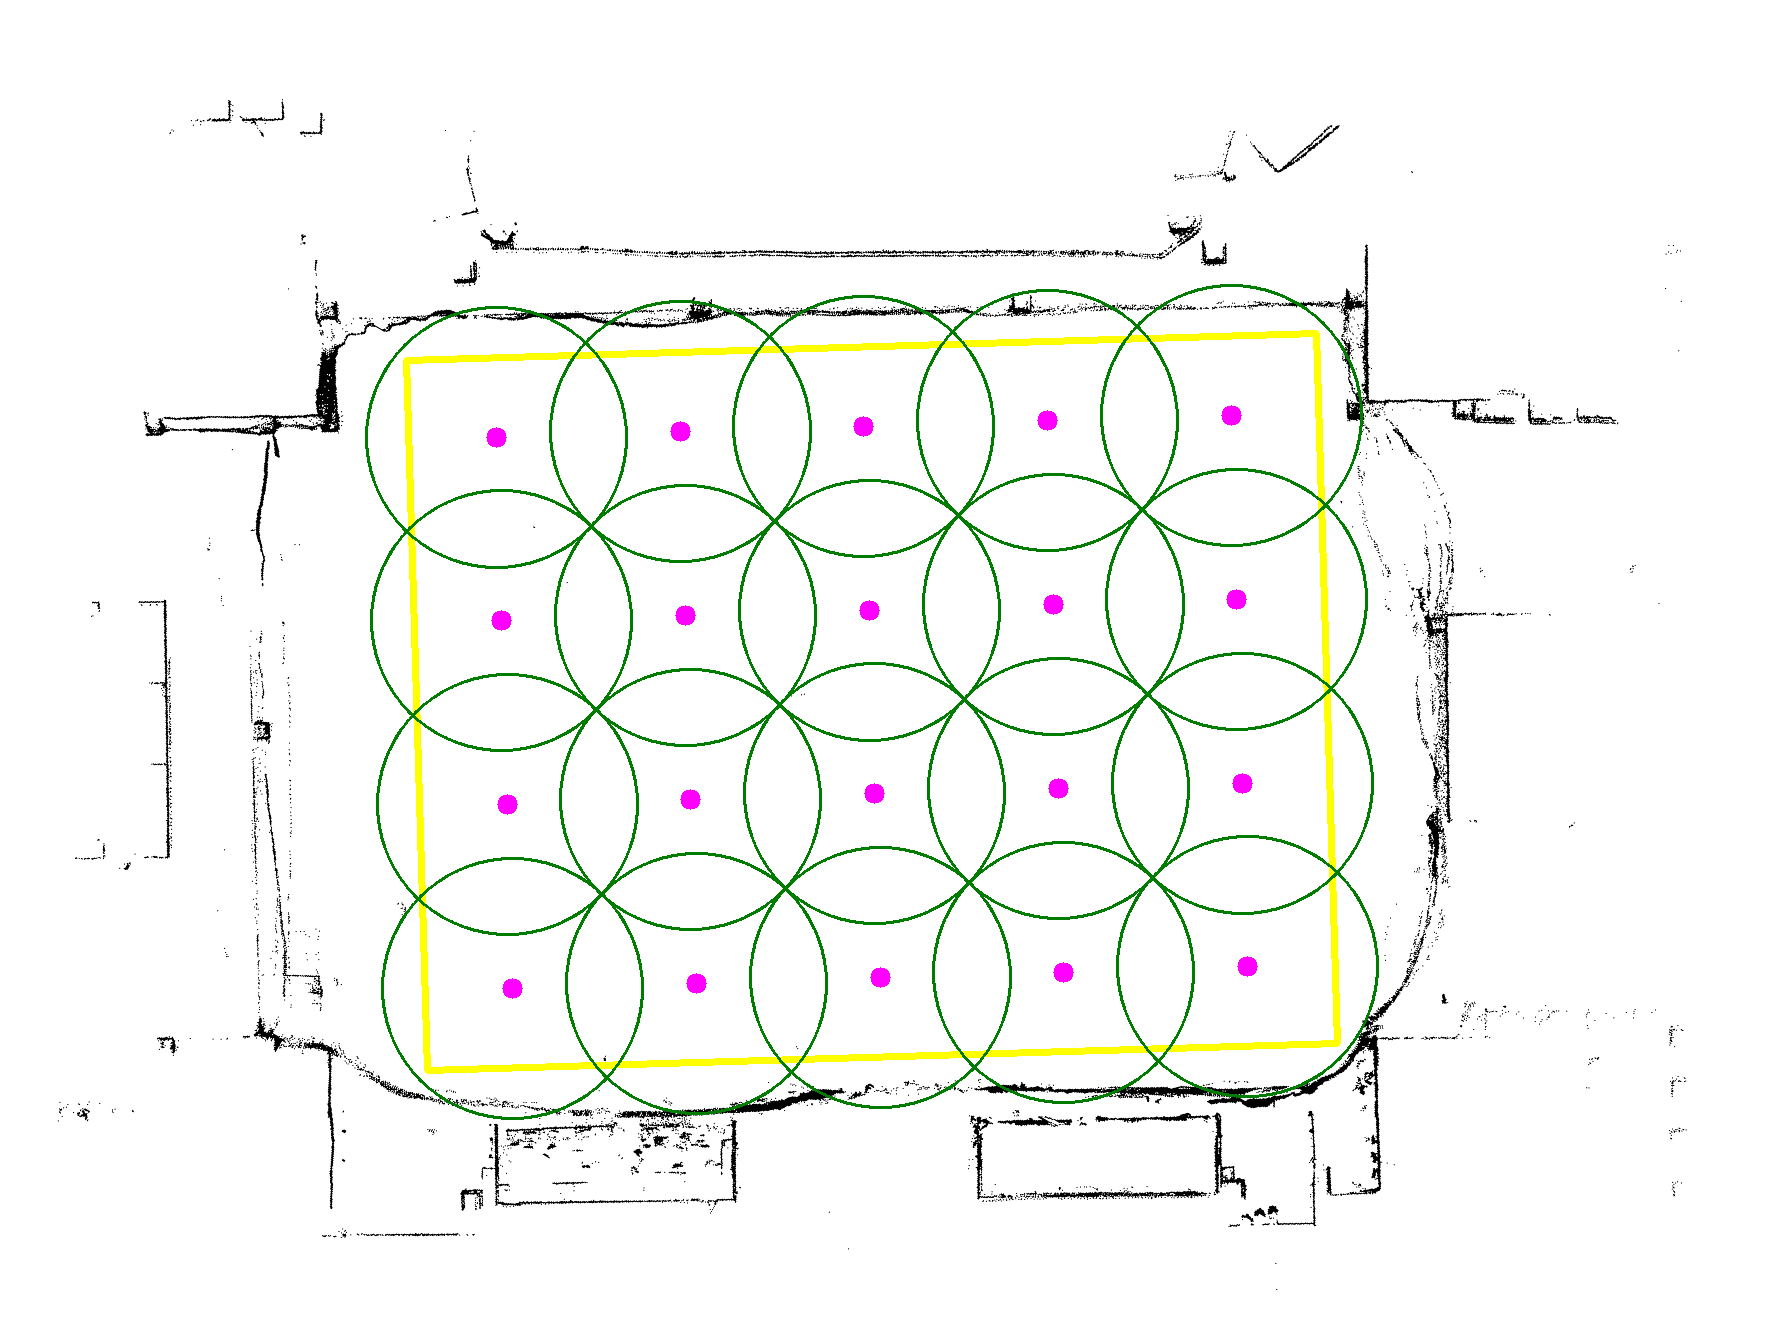
\includegraphics[scale=0.25]{fig/map_annotation.png}
	\caption[Generated waypoints]{Purple waypoints are places where the robot should stop and look around. Green circles are camera ranges from the corresponding place. In this figure are the waypoints generated so that there is no unexplored area. That is usually not necessary since the objects of interest have non-negligible size. It is thus possible to further reduce the number of waypoints.}
	\label{fig:map_annot}
\end{figure}

\begin{algorithm}[H]
	\KwData{waypoints}
	done = False\;
	\While{not done}{
		waypoint = waypoints.pop()\;
		start\_lidar\_detection()\;
		go\_to(waypoint)\;
		stop\_lidar\_detection()\;
		raise\_arm()\;
		do\_camera\_detection()\;
		\If{has\_all\_objects or waypoints.empty()}{
			done = True\;	
		}
	}
	\If{not has\_all\_objects}{
		go\_to(get\_strongest\_candidate())\;
	}
	\caption{Algorithm to explore whole map. The waypoints are ordered prior to this algorithm. How to order them is beyond the scope of this thesis. In algorithm is visible that the method \textbf{start\_lidar\_detection} is non-blocking service which just turns on the detector, whereas the method \textbf{do\_camera\_detection} is blocking service which waits until the arm looks around with camera and finishes the detection. This method is also the most time consuming part of the loop.}
	\label{alg:exploration}
\end{algorithm}

\section{Stacked bricks detection}
It is obvious that, when the bricks are stacked close to each other without any significant gap, it is impossible to distinguish which bricks the lidar detects. This issue was already addressed in previous chapters. It is desired to know what color particular lidar point has. This is done by camera to lidar registration. Since we know the relative position of camera to lidar and also the intristic camera matrix, it is not problem to assign color to each point. The colors are further utilized during the clustering. We can now split clusters not only using the spatial data but the splitting can be based on color difference of subsequent points. Modified clustering is visible in algorithm \ref{alg:clustering}. Note that the color distance is computed from whole cluster mean to a new point. When the new point is added, the color of cluster should be recalculated. This is important to reduce camera noise influence on final form of clusters. When the running mean technique is used, the clusters are split only in sharp color transitions. How the pointcloud coloring and final detection looks like is shown in the figure  \ref{fig:colors}. Since the robot stacked all of these bricks, their relative position should be known. Whole stacking is predefined sequence of movements and thus we can add each placed brick into the list of stacked bricks with its relative position to place where stacking started. These known positions can be used to generate hypothesis which can be fitted with the RANSAC algorithm in the same way as during the pattern fitting. When we use colors for the segmentation, it is important to choose right color space. During the experiments was much easier to distinguish between green and blue color in LAB color space than in HSV color space. The robot is not capable of carrying orange bricks so that it was not necessary to segment also the orange color which is problematic, because it can be easily confused with red color. This part of detection is not discussed any further because it was more important to localize initial position of UGV bricks and placing more than one load of bricks was not achievable in given timeframe.

\begin{algorithm}[H]
	\KwData{points}
	\KwResult{clusters}
	initialize constants C, T, min\_size \;
	cluster = []\;
	clusters = []\;
	\ForEach{pt in points}{
		\eIf{cluster.empty()}{
			cluster.push\_back(pt)\;
		}{
			\eIf{distance(pt, cluster[end]) $<$ C and color\_distance(pt, cluster) $<$ T}{
				cluster.push\_back(pt)\;
			}{
				\If{cluster.size() $>$ min\_size}{
					clusters.push\_back(cluster)\;
				}
				cluster.clear()\;
			}
		}
	}
	\caption{Spatial and color clustering. Input points must be ordered layer from lidar pointcloud. Constant \textbf{C} is clustering distance, \textbf{T} is color clustering distance and \textbf{min\_size} is minimal cluster size - this has high influence on range of brick candidate generation.}
	\label{alg:clustering}
\end{algorithm}

\begin{figure}[H]
	\centering
	\begin{subfigure}{1\textwidth}
		\centering
		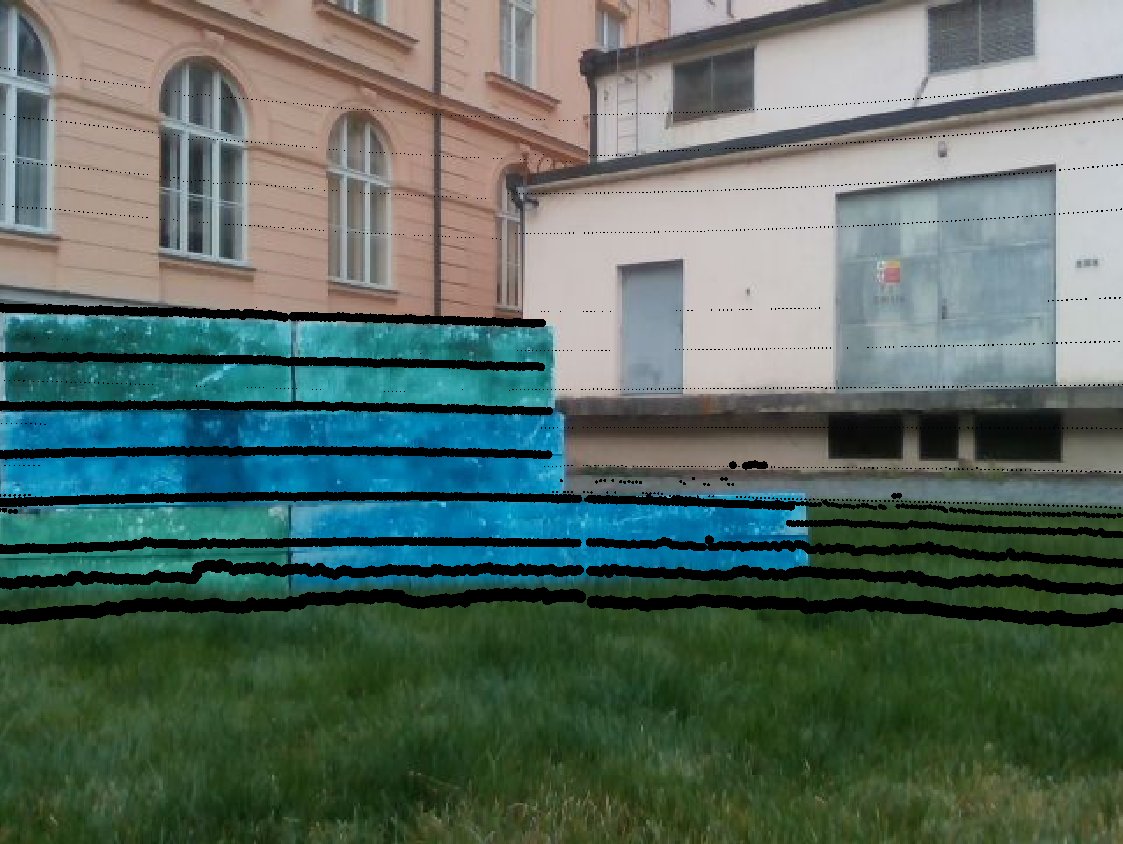
\includegraphics[scale=0.28]{fig/colors_camera}
	\end{subfigure}

	\vspace{5mm}

	\begin{subfigure}{1\textwidth}
		\centering
		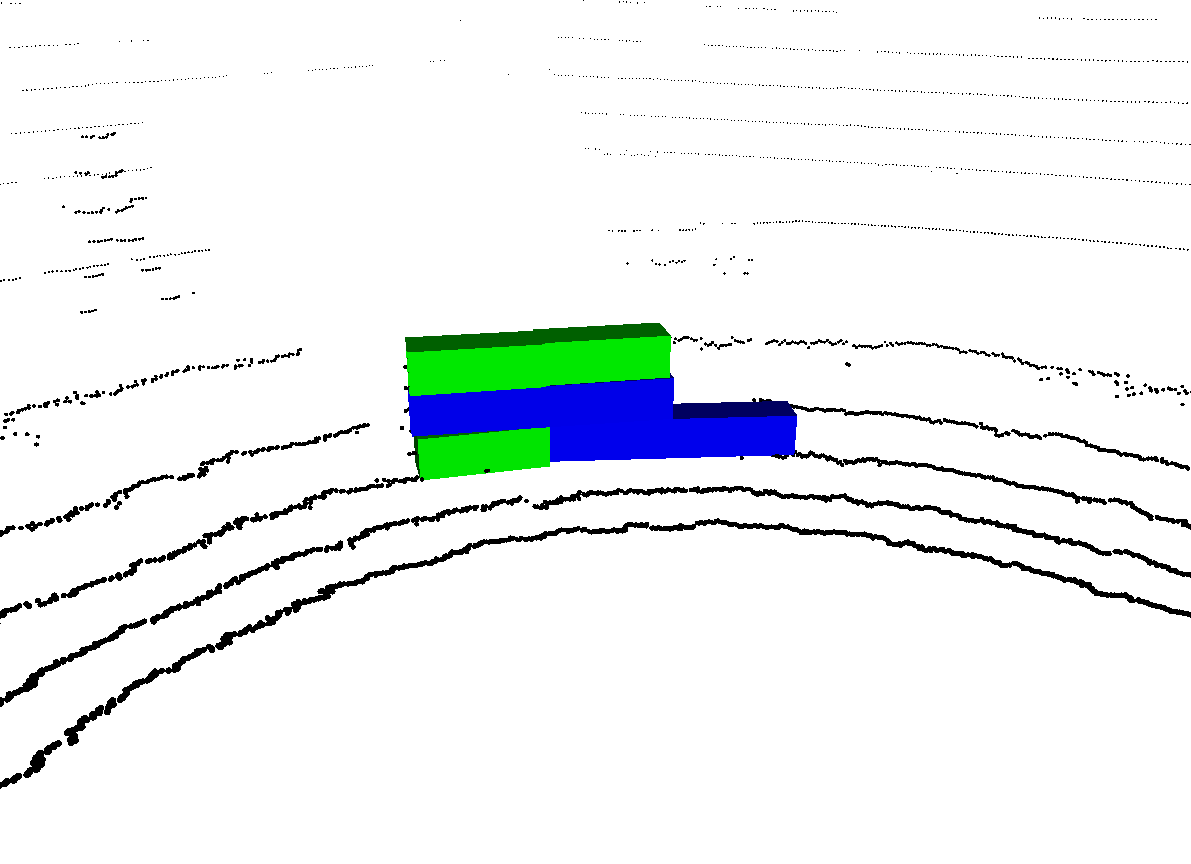
\includegraphics[scale=0.27]{fig/colors_lidar}
		
	\end{subfigure}
	
	\caption[Colored pointcloud detections]{Detection of bricks using color based clustering. At the top is image from camera pointing at built wall. Black dots are points captured by the lidar sensor. At the bottom is shown final detection in map frame. All of the bricks are correctly detected, although they are poorly painted and the environment is quite challenging, especially with the green grass on the ground.}
	\label{fig:colors}
\end{figure}

\newpage
